\section{Zadanie 2}
 Rozpoczynaj�c z punktu pracy - przy zerowym zak��ceniu - wyznaczyli�my trzy odpowiedzi skokowe toru zak��cenie-wyj�cie, wykonuj�c skoki sygna�u zak��caj�cego w chwili $k=0$ odpowiednio do warto�ci 10, 20 i 30. Wszystkie odpowiedzi przedstawione s� na rysunku $Rys. 2.1$.
\begin{figure}[tb]
\centering
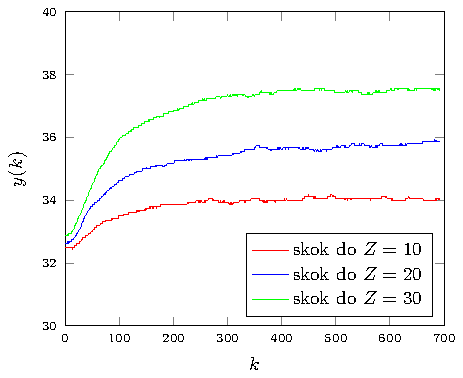
\includegraphics[scale=1]{rysunki/zad2plot}
\caption{Odpowiedzi skokowe toru zak��cenie-wyj�cie dla r�nych zmian sygna�u zak��caj�cego w chwili $k=0$}
\end{figure}
Wyznaczono charakterystyk� statyczn� ($Rys. 2.2.$). W�a�ciwo�ci statyczne obiektu mo�emy okre�li� jako (w przybli�eniu) liniowe.  Wzmocnienie statyczne dla tego toru wynosi w przybli�eniu $\num{0,15}$ - warto�� wsp�czynnika kierunkowego funkcji liniowej b�d�cej charakterystyk� statyczn�.
\begin{figure}[tb]
\centering
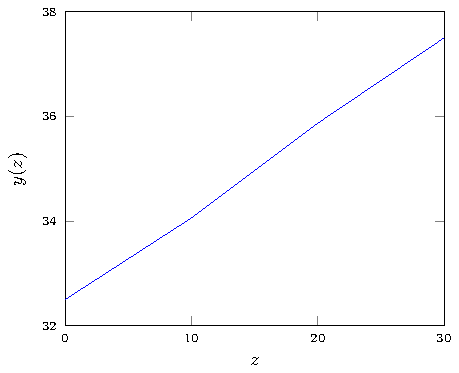
\includegraphics[scale=1]{rysunki/zad2char_st}
\caption{Charakterystyka statyczna - tor zak��cenie-wyj�cie}
\end{figure}